\documentclass[english, 11pt]{report}

\usepackage{babel}
\usepackage{graphicx}
\usepackage{times}
\usepackage{pifont}
\usepackage{geometry}
\usepackage{eurosym}
\usepackage{fancyhdr}
\usepackage[hidelinks]{hyperref}
\usepackage{framed}
\usepackage[thinlines]{easytable}
\usepackage{enumitem}
\usepackage{float}
\usepackage{lastpage}
\restylefloat{table}

\pagestyle{fancy}
\fancyhf{}


%HEADER
%**************************************************************************************
\pagestyle{fancy}
\fancyhf{}
%**************************************************************************************
\lhead{Savonia UAS}		 	 
\rhead{Bachelor's Thesis} 
\cfoot{\thepage}
%**************************************************************************************

\date{}
\setlength\parindent{0pt}

\begin{document}


\nopagebreak
\begin {flushleft}

\includegraphics{savonia.jpg}
\end{flushleft}
\begin {center}
\vspace{2.5in}\Huge Implementation of volume rendering in C\#\\ for LightningChart\\
\vspace{1cm}
 Alexey Tukalo\\
 \vspace{0.5cm}
\small Bachelor's Thesis\\
\vspace{2.1in}
\today \hspace{0.5cm} \noindent\rule{4cm}{0.4pt}
\end{center}
\begin {flushleft}
\large Bachelor’s degree (UAS)
\end{flushleft}
\thispagestyle{empty}

\vspace{2.5in}

\date{\today}


\newpage
\setcounter{page}{1}
\setcounter{tocdepth}{2}

\begin{table*}[!h]
\begin{tabular}{| l | l | l | l |}
\multicolumn{2}{l}{\textbf{SAVONIA UNIVERSITY OF APPLIED SCIENCES}}&
\multicolumn{2}{r}{\textbf{THESIS}}\\
\multicolumn{4}{r}{\textbf{Abstract}}\\
\hline
\multicolumn{4}{|l|}{Field of Study}\\
\multicolumn{4}{|l|}{Technology, Communication and Transport}\\
\hline
\multicolumn{4}{|l|}{Degree Programme}\\
\multicolumn{4}{|l|}{Degree Programme in Information Technology}\\
\hline
\multicolumn{4}{|l|}{Author}\\
\multicolumn{4}{|l|}{Alexey Tukalo}\\
\hline
\multicolumn{4}{|l|}{Title of Thesis}\\
\multicolumn{4}{|l|}{Implementation of volume rendering in C\# for LightningChart}\\
\hline
Data & \today & Pages/Appendices & \pageref{LastPage}\\
\hline
\multicolumn{4}{|l|}{Supervisor}\\
\multicolumn{4}{|l|}{Arto Toppinen}\\
\hline
\multicolumn{4}{|l|}{Client Organization/Partners}\\
\multicolumn{4}{|l|}{Arction Oy}\\
\hline
\multicolumn{4}{|l|}{Abstract}\\
\multicolumn{4}{|l|}{ }\\
\multicolumn{4}{|p{14cm}|}{
Arctive Oy is a Finnish software company, based in Kuopio. Their main product is LightningChart, the fastest C\# framework for the visualisation of scientific, engineering, trading and research data. The library contains a bunch of tools for visualisation of XY, 3D XYZ, smith and polar graphs, 3D pie/donut views, 3D objects.
}\\
\multicolumn{4}{|l|}{ }\\
\multicolumn{4}{|p{14cm}|}{
The company wanted to extend the LightingChart's abilities of polygonal 3D models rendering by volume rendering. It gives Arction an opportunity to attract new clients to the product. In result the framework will provide an unique possibility to render volume and polygonal models at same visualisation.
}\\
\multicolumn{4}{|l|}{ }\\
\multicolumn{4}{|p{14cm}|}{
The project started from a literature research and comparison of different volume visualisation techniques, to choose the best one for the Arction's case and implement it inside the framework. The implementation of the volume rendering engine is based on DirectX used together with C\# via SharpDX API and HLSL shader language for low level optimisation of rendering calculations.
}\\
\multicolumn{4}{|l|}{ }\\
\multicolumn{4}{|p{14cm}|}{
The final chapter of the report contains an evaluation of the results and suggestion for a future development of the engine.
}\\
\multicolumn{4}{|l|}{ }\\
\hline
\multicolumn{4}{|l|}{Keywords}\\
\multicolumn{4}{|p{14cm}|}{
Visualisation, Ray Casting, 3D, C\#, LightningChart, DirectX, HLSL, Image Processing, Volume Rendering, Rendering
}\\
\hline
\end{tabular}
\end{table*}

\newpage

ACKNOWLEDGEMENTS\\

I am very thankful to Arction Oy for offering me an opportunity to take part in the development of the project. I really like the office atmosphere and freedom in terms of my working style and schedule allowed by the company.\\

My special thanks goes to Mr. Pasi Toummainen, CEO of the company, who expressed interest in my idea to extend the library by the volume rendering engine, gave me permission to work on the project and guided me especially in the very early part of the development process.\\

Moreover, I would like to say thank you to my supervisor of thesis, Arto Toppinen, for his mentoring and support during the report writing stage of my work. \\

In addition, I would like to express my deepest gratitude Karlsuruhe Institute of Technology, there I got the first experience with volume rendering via Ray Casting. I am especially grateful to Nicolas Tan, Jerome, who was my mentor during the part of my internship related to modification of Tomo Ray Caster 2 and to Aleksandr Lizin, the creator of the volume rendering engine based on WebGL.

\newpage

\tableofcontents

\chapter{Introduction}
This chapter contains brief information about the motivation behind volume rendering, my personal background in computer graphics especially volume rendering. It also introduces Acrtion as the owner of the project, explains the reasons for Arction's interest in the development, set requirements for the final product.
\section{Motivation}

Volume data is very common our day. An importance of the type of datasets will grow in the near future, because of development in the field of 3D data acquisition and possibilities to perform the visualisation of this type of information on a modern office workstation with an interactive frame rate.\\

Volume rendering is a process of multi-dimensional data visualisation into a two-dimensional image which gives the observer an opportunity to recognize meaningful insights in the original information. The technology allows us to represent 3 dimensions of the data via position in a 3D space and 3 more via color of the point.\\

The dataset can be captured by various numbers of technologies like: MRI\footnote{Magnetic resonance imaging}, CT\footnote{Computer tomography}, PET\footnote{Positron emission tomography}, USCT\footnote{Ultrasound computer tomography} or echolocation. They also can be produced by physical simulations, for example fluid dynamics. The set of technologies mentioned before demonstrates that volumetric information plays a big role in medicine. It is used for an advanced cancer detection, visualization of aneurisms and treatment planning. This kind of rendering is also very useful for non-destructive material testing via computer tomography or ultrasound. Geoseismic researches produce huge three-dimensional datasets. Their visualisations are used in an oil exploration and planning of the deposit development.\\
%http://www.labri.fr/perso/preuter/imageSynthesis/02-03/papers/volvistut.pdf

\section{Personal backgound}

I received my first experience in the visualisation of volumetric data during my internship at the Institute of Data Processing and Electronics, which belongs to the Karlsruhe Institute of Technology (KIT). I was a part of the 3D Ultrasound Computer Tomography (USCT) team. Their main goal is the development of a new methodology for early breast cancer detection. During the work placement I had to develop an algorithm to visualise five-dimensional datasets. In result the algorithm was integrated into Tomo Ray Caster 2\footnote{JavaScript framework for the visualisation of 3D data, developed in Institute of Data Processing and Electronics} and USCT's edition of DICOM Viewer.\\

\begin{figure}[H]
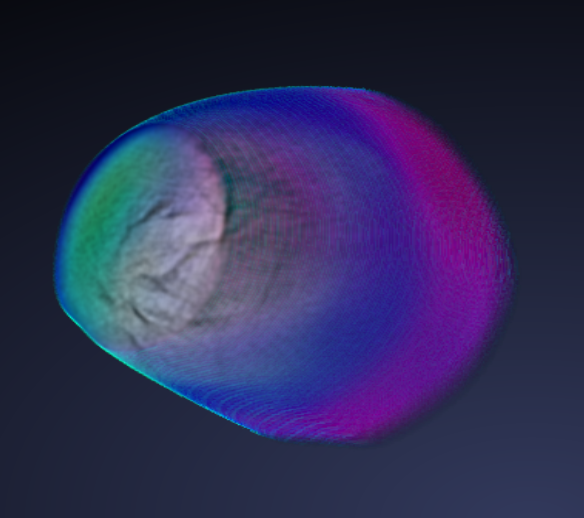
\includegraphics[scale=0.4]{img/usct1}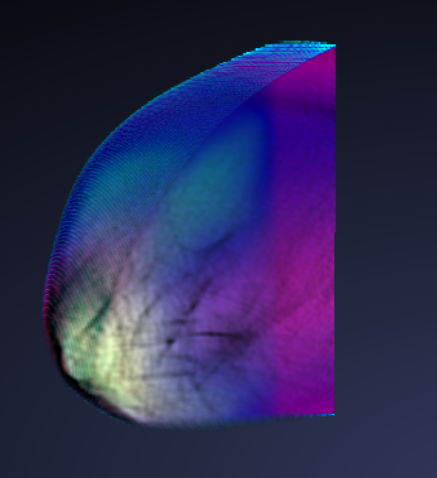
\includegraphics[scale=0.4335]{img/usct2}\\
\caption{Volume visualisation of breast phantom made by USCT}
\end{figure}
%USCT VIS

During the project I made my very first steps in modern computer graphics. I got my first experience in work with WebGL during customisation of the Tomo Ray Caster and learned GLSL as my first shader language. I also gained a lot of knowledge about image processing and scientific data visualisation, which became the basis for my thesis work.

%INTERNSHIP REPORT

\section{Arction Oy and Ligthning Chart}

Arction Oy is a Finnish software company based in Kuopio. Their team has a strong background in computer graphics and science. The main product of the company called LightningChart Ultimate. It is the fastest C\# library for scientific and engineering data visualisation. The library is capable to draw massive XY, Polar, Smith and 3D XYZ graphs, polygonal mesh models, surfaces, 3D pies/donuts and Geographic information. The library has an API for .NET WinForm and WPF applications, it is also possible to use it for a traditional Win32 C++ software development. The main advantage of the library is the fact that it is based on low-level DirectX graphics routines developed by Arction, then the most part of competitors use graphics routines which belongs to System.Windows.Media.\\
\begin{figure}[H]
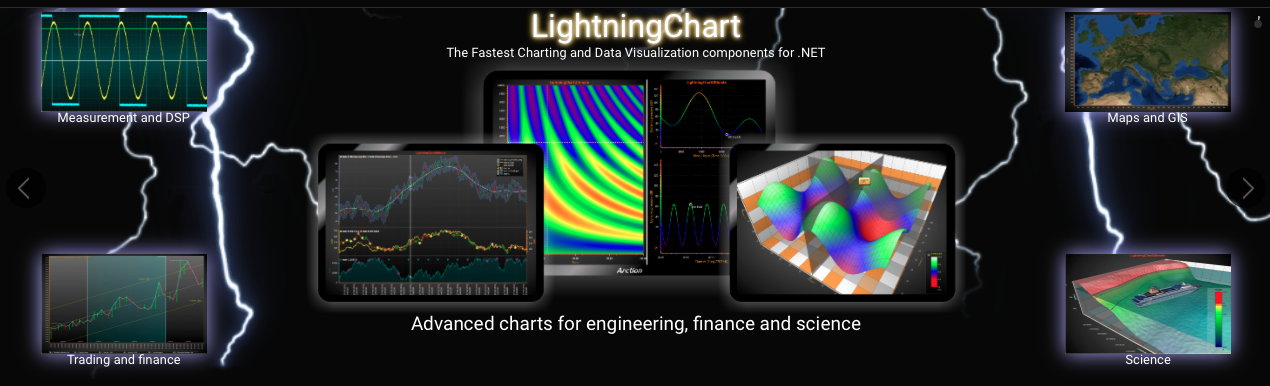
\includegraphics[scale=0.33]{img/lchu}\\
\caption{Example of LightningChart possibilities from the main page of Acrtion}
\end{figure}
%arction website

\section{Project Goals}

So, as you can conclude from the previous section, LightningChart is a very advanced software for 3D rendering based on polygons and lines. That's why, I came up with an idea to extend it by the special rendering engine for visualisation of volumetric data. It will give Arction's clients the unique possibility to combine visualisation of volume datasets with a wide range of other 3D possibilities provided by the library. \\

The rendering engine must be able:
\begin{itemize} 
\item to render large multi-dimensional volumes with an interactive frame rate.
\item to move and rotate the model in the chart's space.
\item to provide clients with possibilities to apply windowing and thresholding to the initial dataset.
\item to render the model semi-transparent.
\end{itemize}

Basically, this tool will give end users possibilities to change the contrast and brightness of the model's visualisation for better recognition of tiny details and make areas, which are out off certain range, totally transparent. It will also reveal insights into the internal structure of the model to the user via semi-transparency.

\chapter{Theory}

This chapter explains the theory behind the project. It should introduce the main concepts of computer graphics, specify the difference between polygonal mesh model and volume rendering. It also contains an overview of different volume rendering techniques with their advantages and disadvantages in terms of speed, final image quality, flexibility and other implementation issues.

\section{Rendering}

Visualisation of 3D object as 2D image called rendering. Usually, 2D image is based on pixels\footnote{a shortcut from picture element}. In case of a grayscale picture, it is a two-dimensional array and the value of the array elements represents the brightness of corresponding pixels on a screen. Configuration of colored images is dependent from a color model, the most popular one is RGB. It represents an image as three different grayscale pictures for three different colors called channels. In case of the RGB color model the images contain Red, Green and Blue values, sometimes it also keeps an informant about opacity and the channel called Alpha.\\

Color model is the mathematical abstraction which allows computers to calculate brightness of a corresponding point on the screen. RGB is the original one for modern computer graphics, because it represents colors in the way they are physically reproduced on screen. There are several other color models. They have their own advantages, for example, some of them gives us an advanced editing possibilities while others represent physical characteristic of different types of output devices like printers.\\

Multidimensional data can be represented in two different ways: as a surface and as volume. Future in this chapter, we are going to talk about these two concepts a little bit closer. We will highlight their advantage and disadvantages, common and uncommon features. Moreover, we are going to discuss an implementation detail of the techniques on modern hardware.

%https://www.artstation.com/artist/vidarrapp illustration


\section{Polygonal Rendering}

Today we are literally surrounded by the surface rendering based on polygonal mesh. The technology is used in computer games, design, cinema, science, engineering and etc. The technology is so popular that entire 3D graphic pipeline is built around the idea. That's why this type of visualization is easily accelerated by graphic cards.\\

\subsection{Vertexs}
Traditionally, 3D surfaces are constructed out of huge amount of polygons connected as a mesh. Due to simplicity, they usually have a triangular shape. It is possible to describe triangle via list of three coordinates called vertices. The internal area of the shape filled with color during rasterization step. The color is calculated as dot product between the surface vector normal and the vector of light.
%http://people.csail.mit.edu/fredo/Depiction/1_Introduction/reviewGraphics.pdf

\begin{figure}[H]
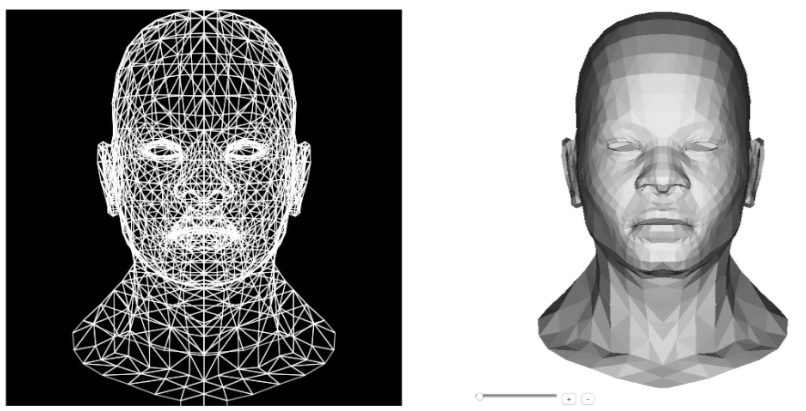
\includegraphics[scale=0.55]{img/mesh}\\
\caption{Wireframe and flat shading polygonal meshmodel}
\end{figure}

\subsection{Normals}
Surface normal vector of a triangle can be calculated as a cross product of two triangle's sides, but it will give an acceptable result only for very flat surfaces. That's why curve surfaces usually contain an additional normal vector for every vertex. They are able to significantly improve detailisation on the model. The information kept in them is used during shading and the tessellation of the model's geometry.\\

%http://www.emeyex.com/site/tuts/VertexNormals.pdf

\subsection{Textures}
Very small details can be added to the model via textures. It is specific 2D image which is used to sample high frequency information during rendering. The picture usually contains local color values, but it also can carry an information about normal vectors for a nice visualisation of very small structures on the surface. Textures are mapped to the surface via third vertex' parameter called texture coordinates. They keep an information about corresponding to this vector position in the 2D space of the image.\\

%http://www.dcs.ed.ac.uk/teaching/cs4/www/graphics/Web/advanced_ogl.pdf

\subsection{Redering process}
Position, scale, rotation of the object and perspective characteristics of the space is specified via matrixes $4\times4$.\\

%http://www.tutorialspoint.com/computer_graphics/3d_transformation.htm

Specific program called shader receives all the information together with a camera and light source positions, after that they are able to perform calculations needed to render the final image in accord with the goals of the visualisation. Usually, the calculations are produced by graphic card in a parallel way.

\section{Volume Rendering}
There are two ways to render volumes. We are going to discuss about main principles, advantages and disadvantages of the technologies in this section.

\subsection{Indirect}

The first one called indirect volume rendering. It is based on the idea that it is possible to extract surface out of the dataset during preprocessing and render the surface as a polygonal mesh. Several algorithms are invented for this application:
\begin{itemize}
\item Marching Cubes
\item Surface Tracking
\item Fourier Transfor Rendering
\end{itemize}
It is the oldest idea behind volume rendering and it has plenty of disadvantages:
\begin{itemize}
\item complex and slow preprocessing algorithms
\item can be inacurate due to noise
\item sometimes does not able to generate isosurface out of specific dataset, for example smoke
\item lose an information about an internal structure
\item need to repeat preprocessing to apply changes in a transfer function
\end{itemize}

But the algorithm is very popular for generation of medical illustrations, video or other static visualisation. The main advantage of the solution is that nicely preprocessed model can be easily rendered in via wel-known 3D mesh models' rendering, even in very weak hardware.\\

Unfortunately, this technology is not suitable for our project, because it does not satisfy our requirements.

%http://www.forceflow.be/wp-content/uploads/2012/02/vr_overview.pdf


\subsection{Direct}
Direct volume rendering does not require any preprocessing. The data visualised from the initial dataset and it gives the algorithms an opportunity to modify the transfer function run time. There are four technics for direct volume rendering based on totally different ideas. Future we are going to discuss about them more detailed.
%http://www.forceflow.be/wp-content/uploads/2012/02/vr_overview.pdf
\subsubsection{Texture-based}
\subsubsection{Ray Casting}
\subsubsection{Splatting}
\subsubsection{Shear-warp}

\chapter{Implementation}
\section{Tools}
\subsection{C\#}
\subsection{DirectX 11}
\subsubsection{Redering Pipeline}
\subsubsection{HLSL}
\subsection{SharpDX}
\subsection{LightningChart Ultimate}
\section{Visualisation process}
\subsection{Loading and preprocessing of dataset}
\subsection{Multi-pass rendering}
\subsubsection{First pass}
\subsubsection{Second pass}
\paragraph{Empty space skipping}
\paragraph{Ray function}

\chapter{Conclusion}
\section{Results}
\subsection{Rotation and position}
\subsection{Settings}
\subsubsection{Windowing}
\subsubsection{Thresholding}
\subsubsection{Slice range clipping}
\subsection{Mouse picking}

\section{Disscusion}

\section{Future Development}

\chapter{Appendix}








\end{document}
